\documentclass[10pt,a4paper]{article}
\usepackage[utf8]{inputenc}
\usepackage{amsmath}
\usepackage{amsfonts}
\usepackage{amssymb}
\usepackage{graphicx}
\usepackage{float}
\usepackage[hidelinks]{hyperref}
\usepackage[left=1in,right=1in,top=1in,bottom=1in]{geometry}

\title{Pipeline control protocol for the Otter MCU}
\author{Trevor McKay}
\date{Summer 2020}

\graphicspath{{./figures/}}

\begin{document}

\begin{center}
    \Large\textbf{RISC-V UART Debugger\\Protocol and Implementation}

    \medskip
    \small{for CPE-233 and CPE-333 at Cal Poly, SLO}

    \bigskip
    \tiny{Trevor McKay}
\end{center}

\tableofcontents

\newpage
\section{Quickstart}
If you are just looking to get up and running as fast as possible, start here. Thankfully, the
protocol is not very complex despite this document's size. It contains a lot of detail so that there
is no ambiguity in how the module should be implemented. However, most of implementation is very
straight forward. Here is an outline of what needs to be done to get the debugger working on your Otter:

\begin{enumerate}
    \item Clone the repository.
    \item Add the files in \emph{module/design} to the Otter Vivado project.
    \item Add logic variables for \emph{pause}, \emph{resume}, \emph{valid}, etc.
    \item Add \emph{srx} as an input and \emph{stx} as an output to the wrapper and MCU.
    \item Instantiate and connect the \emph{mcu\_controller} module in the MCU.
    \item Give your MCU the ability to pause, resume, reset, and read and write per the protocol.
    \item Install the client.
    \item Run the client with \emph{uart-db}.
\end{enumerate}

\noindent Return to this document for more clarification on any of the above steps.

\section{General overview of module and protocol}

\subsection{Overview}

This protocol aims to make hardware add-ons and software for your Otter easier to develop. Control flow operations
allow for easy manipulation of the state of the CPU as well as many low-level operations such


Return to this document for more clarification on any of the above steps.as memory and register editing, pause, or resume. Fortunately, all debugging operations can be
implemented with commands or a series of commands added by implementing this
protocol.

\medskip
\noindent\underline{\href{https://github.com/trmckay/riscv-uart-debugger}{Code repository}}

\subsection{Connections}

\begin{figure}[H]
    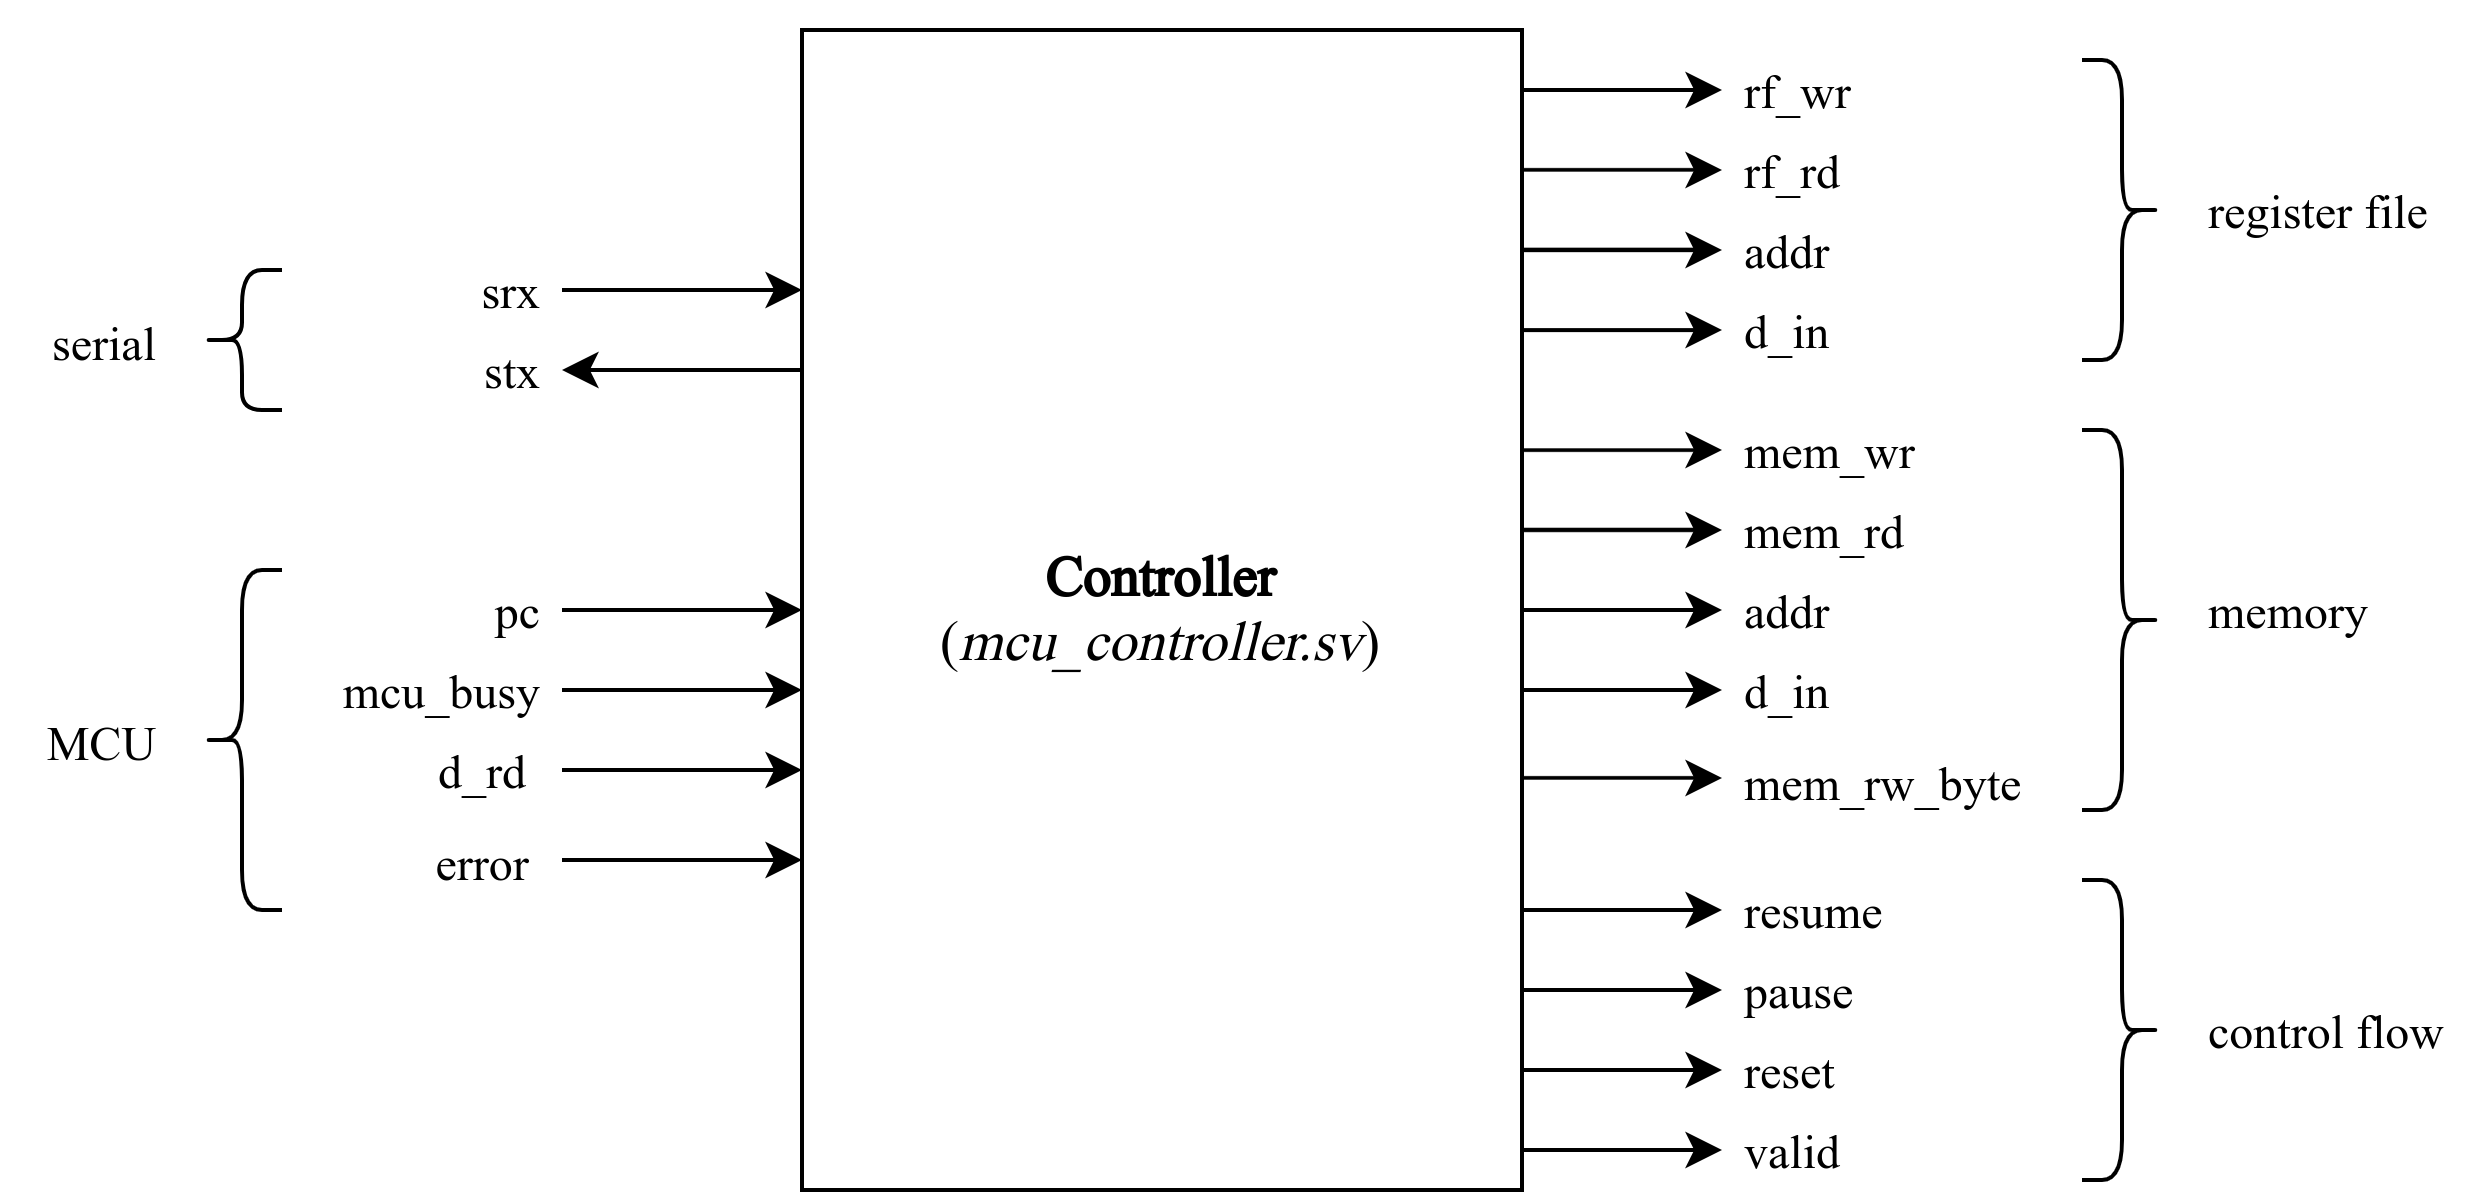
\includegraphics[width=\textwidth]{blackbox}
\end{figure}
\medskip

The module connects to the MCU, register file, and memory. Commands are recieved via serial
and decoded within the module. The signals \emph{rf\_wr}, \emph{rf\_rd}, \emph{addr}, and
\emph{d\_in} connect to the register file for reads and writes. The \emph{mem\_wr},
\emph{mem\_rd}, \emph{mem\_rw\_byte}, \emph{addr}, and \emph{d\_in} connect to the memory
for reads and writes. Additionally, \emph{resume}, \emph{pause}, and \emph{reset} control
the flow of the MCU\@. Finally, the \emph{valid} signal determines wether or not the controller
is issuing a command.

\subsection{Protocol}

It can be assumed that reads, writes, and resumes will only be issued while the MCU is paused. It
can also be assumed that only one command will occur at any time. If any two commands are issued at the
same time, it may be helpful to set \emph{error} and perhaps even do some handling.

\begin{enumerate}

    \item\textbf{valid}\\
    Indicates that the debugger is issuing a command. The MCU should respond accordingly on the next
    positive clock edge. However, \emph{mcu\_busy} should be asserted immediately so that the
    controller goes into the waiting state on the next cycle. The \emph{valid} signal is one-shot;
    however, control signals such as \emph{pause} and \emph{resume} will be held until the MCU is
    finished.

    \item\textbf{resume}\\
    The MCU should resume normal operation. If this takes more than one cycle,
    keep \emph{mcu\_busy}high to indicate this.

    \item\textbf{pause}\\
    The MCU should appear to stop execution after the current instruction completes. The
    \emph{mcu\_busy} signal should be asserted as soon as \emph{pause} and \emph{valid} are both
    high. For multicycle MCUs, the MCU should not fetch any more instructions (this can be done by
    injecting \emph{no-op}s) once the pause begins. Only when the current instruction has committed
    all of its changes should \emph{mcu\_busy} go low. Pipelined MCUs will also need to halt
    instruction fetching, but will additionally need to flush the pipeline of all partially completed
    instructions. Once again, \emph{mcu\_busy} should only go low once the flush is completed.

        \begin{verbatim}
                 clk:  __|¯¯|__|¯¯|__|¯¯|__|¯¯|__|¯¯|__|¯¯

            mcu_busy:  ______________|¯¯¯¯¯¯¯¯¯¯¯|_________

               pause:  ______________|¯¯¯¯¯¯¯¯¯¯¯|_________

               valid:  ______________|¯|___________________
        \end{verbatim}

    \item\textbf{reset}\\
    The program counter should be set to zero. It is worth noting that this only resets the point of
    execution, not the contents of memory.

    \item\textbf{mem\_be}\\
    This signal will be driven high at the same time as \emph{mem\_rd} or \emph{mem\_wr}. It acts as
    a bitmask for selecting bytes from a word. For example, if writing to address 0x14 with
    \emph{mem\_be} as $1111_{2}$, the whole word should be written (addresses 0x14--0x17).
    Reads and writes can be performed at the byte level by using the
    bitmask. For example, accessing word 0x14 with \emph{mem\_be} as $0010_{2}$ will
    only write the third byte in the word (address 0x16).

    \newpage
    \item\textbf{mem\_rd}\\
    The MCU should read the memory at \emph{addr}. The \emph{mcu\_busy} should go
     high at or before the next positive clock edge until the memory read is complete. The
    controller will attempt to read the data \emph{d\_rd} on the first positive clock edge that
    \emph{mcu\_busy} is low. If the address is out of range, set \emph{error} to high.

        \begin{verbatim}
                 clk:  __|¯¯|__|¯¯|__|¯¯|__|¯¯|__|¯¯|__|¯¯

            mcu_busy:  ________|¯¯¯¯¯¯¯¯¯¯¯¯¯¯|___________

                d_rd:  <______ Z ____________><__ 0x17 __>

              mem_rd:  ________|¯¯¯¯¯¯¯¯¯¯¯¯¯¯|___________

               valid:  ________|¯|________________________
        \end{verbatim}

    \item\textbf{mem\_wr}\\
    The MCU should write the data \emph{d\_in} to the memory at \emph{addr}. The \emph{mcu\_busy}
    should go high at or before the next positive clock edge until the memory write is complete.

        \begin{verbatim}
                 clk:  __|¯¯|__|¯¯|__|¯¯|__|¯¯|__|¯¯|__|¯¯

            mcu_busy:  ______________|¯¯¯¯¯¯¯¯¯¯¯|________

                d_in:  <_________ 0x17 __________><_ Z __>

              mem_wr:  ______________|¯¯¯¯¯¯¯¯¯¯¯|________

               valid:  ______________|¯|__________________
        \end{verbatim}

    \item\textbf{rf\_rd}\\
    The MCU should read the register file at \emph{addr}. The \emph{mcu\_busy} signal should go
    high at or before the next positive clock edge until the read is complete. However, it is
    likely that the register file supports asynchronous reads. If this is the case, and the data
    will be ready on the following clock edge, \emph{mcu\_busy} does not need to be asserted.

        \begin{verbatim}
                 clk:  __|¯¯|__|¯¯|__|¯¯|__|¯¯|__|¯¯|__|¯¯

            mcu_busy:  ___________________________________

                d_rd:  <_____ Z ____><______ 0x17 _______>

              reg_rd:  _________|¯¯¯¯|____________________

               valid:  _________|¯|_______________________
        \end{verbatim}

    \newpage

    \item\textbf{rf\_wr}\\
    The MCU should write the data \emph{d\_in} to the memory at \emph{addr}. The \emph{mcu\_busy}
    should go high at or before the next positive clock edge until the memory write is complete.
    This should only take one cycle for the register file; if so, \emph{mcu\_busy} will not need to
    be asserted.

        \begin{verbatim}
                 clk:  __|¯¯|__|¯¯|__|¯¯|__|¯¯|__|¯¯|__|¯¯

                  pc:  <_____________ 0x0C ______________>

            mcu_busy:  ___________________________________

                d_in:  <________ 0x17 _____><_____ Z ____>

              reg_wr:  ______________|¯¯¯¯¯¯|______________

               valid:  ______________|¯|___________________
        \end{verbatim}

\end{enumerate}

\section{Implementation on the Otter}
The protocol aims to standardize things to some extent, but implementation still varies from archictecture
to architecture. The first step is, of course, to clone or download the \emph{.sv} files in the
repository linked at the beginning of the document. All necessary files are located in
\emph{module/design}. Then instantiate the \emph{mcu\_controller} module (\emph{mcu\_controller.sv})
in your MCU. Connect all the inputs and outputs, perhaps designating the outputs as
\emph{ctrlr\_<name>} to differentiate them from similar signals.

\subsection{Some notes on clock speed, baud, connection quality}
By default, the module is instantiated for a clock speed of 50 MHz. If your MCU does not operate at
this speed, you must overwrite this parameter, or the serial connection will be out of sync. The
parameter is set as \emph{CLK\_RATE = x}, where \emph{x} is an integer representing the clock rate
in MHz. Non-integer clock speeds may work, but there is a higher likelihood of desynchronization.
There is a testbench \emph{db\_wrapper} that will act as a target MCU for the debugger. One can
generate a bitstream for this module and connect to it with the client to test it out the connection
and sofware before implementing it on your own Otter.

\subsection{Multicycle Otter (CPE-233)}

\subsubsection{Pausing}
There are two different times the controller can issue a pause command. The simplest to handle is
when the Otter is in the instruction fetch state. The second, more complicated, case is if the pause
command is recieved in the execute or writeback states.

For the following code snippets, assume that \emph{ctrlr\_pause} and \emph{ctrlr\_valid} both come from the
controller, the present state of the MCU is determined by \emph{present\_state}.

We can also define registers \emph{pause\_pending} and \emph{paused} to keep track of
needing to pause when possible or being paused, respectively.

One might place the following snippet in their FSM, for example.

\begin{verbatim}
    reg pause_pending = 0;
    reg paused = 0;

    always_ff @(posedge clk) begin
        if ((ctrlr_pause && ctrlr_valid) || pause_pending)
            case(present_state)
                FETCH: begin
                    paused <= 1;
                    pause_pending <= 0;
                end
                EXECUTE: begin
                    pause_pending <= 1;
                end
                WRITEBACK: begin
                    pause_pending <= 1;
                end
                default: begin
                    pause_pending <= 1;
                end
            endcase
    end
\end{verbatim}

This would save a pause signal when it couldn't be immediately completed, then execute a
pause in the fetch state.

As for making sure the MCU appears paused after the pause is executed:

\begin{verbatim}
    always_comb
        pc_ld = !(paused || pause_pending || (ctrlr_pause && ctrlr_valid));
\end{verbatim}

This would have the affect of keeping the program counter paused until the register is cleared.

There is one final issue to deal with. Without intervention, the Otter will fetch and execute the
instruction indefinitely. One can counteract this by ensuring that the Otter does not leave the
instruction fetch state while it is paused.

Both the \emph{pc\_ld} and state machine pausing should be controlled by the \emph{paused} register.

\subsubsection{Resuming}
The motivation for keeping the MCU paused by a single register is that resuming becomes trivial.
Simply set \emph{paused} to zero when a valid resume command is recieved. See the example code
below (assume \emph{resume} comes from the debug controller):

\begin{verbatim}
    always_ff @(posedge clk)
        paused <= (resume && valid) ? 0 : paused;
\end{verbatim}

\subsubsection{Fulfilling reads and writes}
The debug controller will also send request for reads and writes to the Otter. It can be assumed
that these requests will only be issued while the MCU is paused, so it is easy to determine when the
Otter should use its own decoded address and data or the address and data from the debug controller.

Assume that the decoder outputs and \emph{dec\_rs1\_addr} as the register number, \emph{rs1} is an
output from the register file, \emph{alu\_out} is the result from the ALU,
\emph{mem\_addr} is the address of memory that will be written to, \emph{mem\_d\_in} is
the data that will be written to memory, \emph{ctrl\_addr} is the address output from the
debug controller, and \emph{ctrlr\_d\_in} is the data output from the debug controller. This logic
will use the correct address and data depending on the state of the MCU:

\begin{verbatim}
    always_comb begin
        if (paused) begin
            mem_addr  = ctrlr_addr;
            rs1_addr  = ctrlr_addr;
            mem_d_in  = ctrlr_d_in;
            rf_d_in   = ctrlr_d_in;
        end
        else begin
            mem_addr  = alu_out;
            rs1_addr  = dec_rs1_addr;
            mem_d_in  = rs1;
            rf_d_in   = alu_out;
        end
    end
\end{verbatim}

Finally, to actually perform the reads and writes, consider the following code using existing
signals in the FSM (\emph{ctrlr\_} signals come from the debug controller):

\begin{verbatim}
    always_ff @(posedge clk) begin
        if (paused && ctrlr_mem_rd && ctrlr_valid)
            mem_rd2 = 1;
        else if (paused && ctrlr_mem_wr && ctrlr_valid)
            mem_wr = 1;
        else if (paused && ctrlr_rf_wr && ctlr_valid)
            rf_wr = 1;
    end
\end{verbatim}

One should also be sure to connect \emph{mem\_dout2} and \emph{rf\_dout} to the \emph{d\_rd} port of
the controller. Since the command signals other than valid will stay high until the read is
completed, one can select them using said signals.

\begin{verbatim}
    mcu_controller(
        // other connections
        .d_rd((ctrlr_rf_rd) ? rs1 : mem_dout2)
    );
\end{verbatim}

The last aspect of the protocol that must be implemented is asserting \emph{mcu\_busy} when the
Otter is busy completing a debug command. For this architecture, there are two scenarios in which a
command will not be completed in a single cycle: pausing during execute or writeback and
reading/writing memory. The first case, pausing, is easy to handle. If one implements the \emph{pause\_pending}
signal as described above, the Otter is busy when \emph{pause\_pending} is high.

\begin{verbatim}
    logic busy;
    mcu_controller(
        // other connections
        .mcu_busy(busy)
    );

    assign mcu_busy = pause_pending;
\end{verbatim}

This takes care of the pause case, but one must also handle reading/writing memory. Since this operation
always takes exactly one clock cycle, one can use a one-bit register to wait a cycle. The following
code accomplishes this:

\begin{verbatim}
    reg r_wait = 0;

    always_ff @(posedge clk) begin
        if (valid && (ctrlr_mem_rd || ctrlr_mem_wr))
            r_wait <= 1;
        else
            r_wait <= 0;
    end

    assign busy = wait;
\end{verbatim}

If one were to use both techniques as described above, \emph{busy} will be determined by the logical
OR of both.

\begin{verbatim}
    assign busy = wait || pause_pending;
\end{verbatim}

Finally, the UART signals, \emph{srx} and \emph{stx}, must be connected to the debug controller
module. Since they come from the board itself, the signals must be added to the constraints,
wrapper, and MCU, as well. Adding the proper inputs and outputs is simple enough. Assuming the
signals are named \emph{srx} and \emph{stx} in the wrapper, the relevent constraints would be:

\begin{verbatim}
    ##USB-RS232 Interface
    set_property PACKAGE_PIN B18 [get_ports srx]
        set_property IOSTANDARD LVCMOS33 [get_ports srx]
    set_property PACKAGE_PIN A18 [get_ports stx]
        set_property IOSTANDARD LVCMOS33 [get_ports stx]
\end{verbatim}

You will almost certainly need to make changes to all of the code snippets above to match your own
naming conventions and architecture. This is not meant to be cut-and-paste but rather a starting
point for your own implementation.

\subsection{Pipelined Otter (CPE-333)}

\small\emph{Note: read the multicycle Otter implementation section first; it contains crucial information that is not
reiterated here.}

\medskip

\noindent As is the case with most things, implementation for the pipelined Otter is a bit more involved. The
key difference comes in the pause command. In order for coherency to be maintained between the data
read by the debugger and the state of the MCU, pauses must be executed after all partially completed
instructions are finished. In other words, if the MCU is paused at program count \emph{0x10}, it
must appear that the instructions at \emph{0x0}, \emph{0x4}, ..., and \emph{0xC} have fully
executed.

\subsubsection{Flushing, then pausing}
One could introduce a convoluted forwarding scheme into their Otter. But, the simplest solution
is likely just to flush the pipeline before pausing. No sample code will be provided for this task,
as it is impossible to provide something that works the multitude of possible pipeline
architectures. However, one might sequence their logic as such:

\begin{enumerate}
    \item Recieve the pause command when \emph{valid} and \emph{pause} both go high and immediately
        assert \emph{mcu\_busy}.

    \item Pause the PC such that it does not increment on the positive clock edge.

    \item Set a register, \emph{paused}, to one.

    \item Squash all subsequent instructions and keep the program counter paused as long as the
        \emph{paused} register is one.

    \item Load a counter with 4, the number of instructions that need to flush.

    \item Additionally assert \emph{mcu\_busy} while the counter is greater than zero.

    \item Decrease the counter by one each time an instruction completes (if you are using the
        variable latency memory, this will not decrease if waiting for a read or write).
\end{enumerate}

When the flush is complete and the counter reaches zero, \emph{mcu\_busy} will go low. The
controller will then take care of responding to the debug client.

\subsubsection{Resuming, reads, and writes}
With pause implemented correctly, resuming becomes trivial. Simply set the \emph{paused} register to
zero when \emph{resume} and \emph{valid} are high at the same time.

There is, however, one additional complication to consider with the variable latency memory. Reads
and writes to memory now take \emph{n} cycles instead of one cycle. However, the memory bus provides
a convienient way to determine if the read or write is complete. Simply assert \emph{mcu\_busy} if
the Otter is completing a flush, or the Otter is waiting one cycle for a register file operation, or
if the memory hub is telling the MCU to hold.

\newpage
\subsubsection{Diagram}
One possible design for the described behavior is pictured here.

\begin{center}
\begin{figure}[htpb]
    \centering
    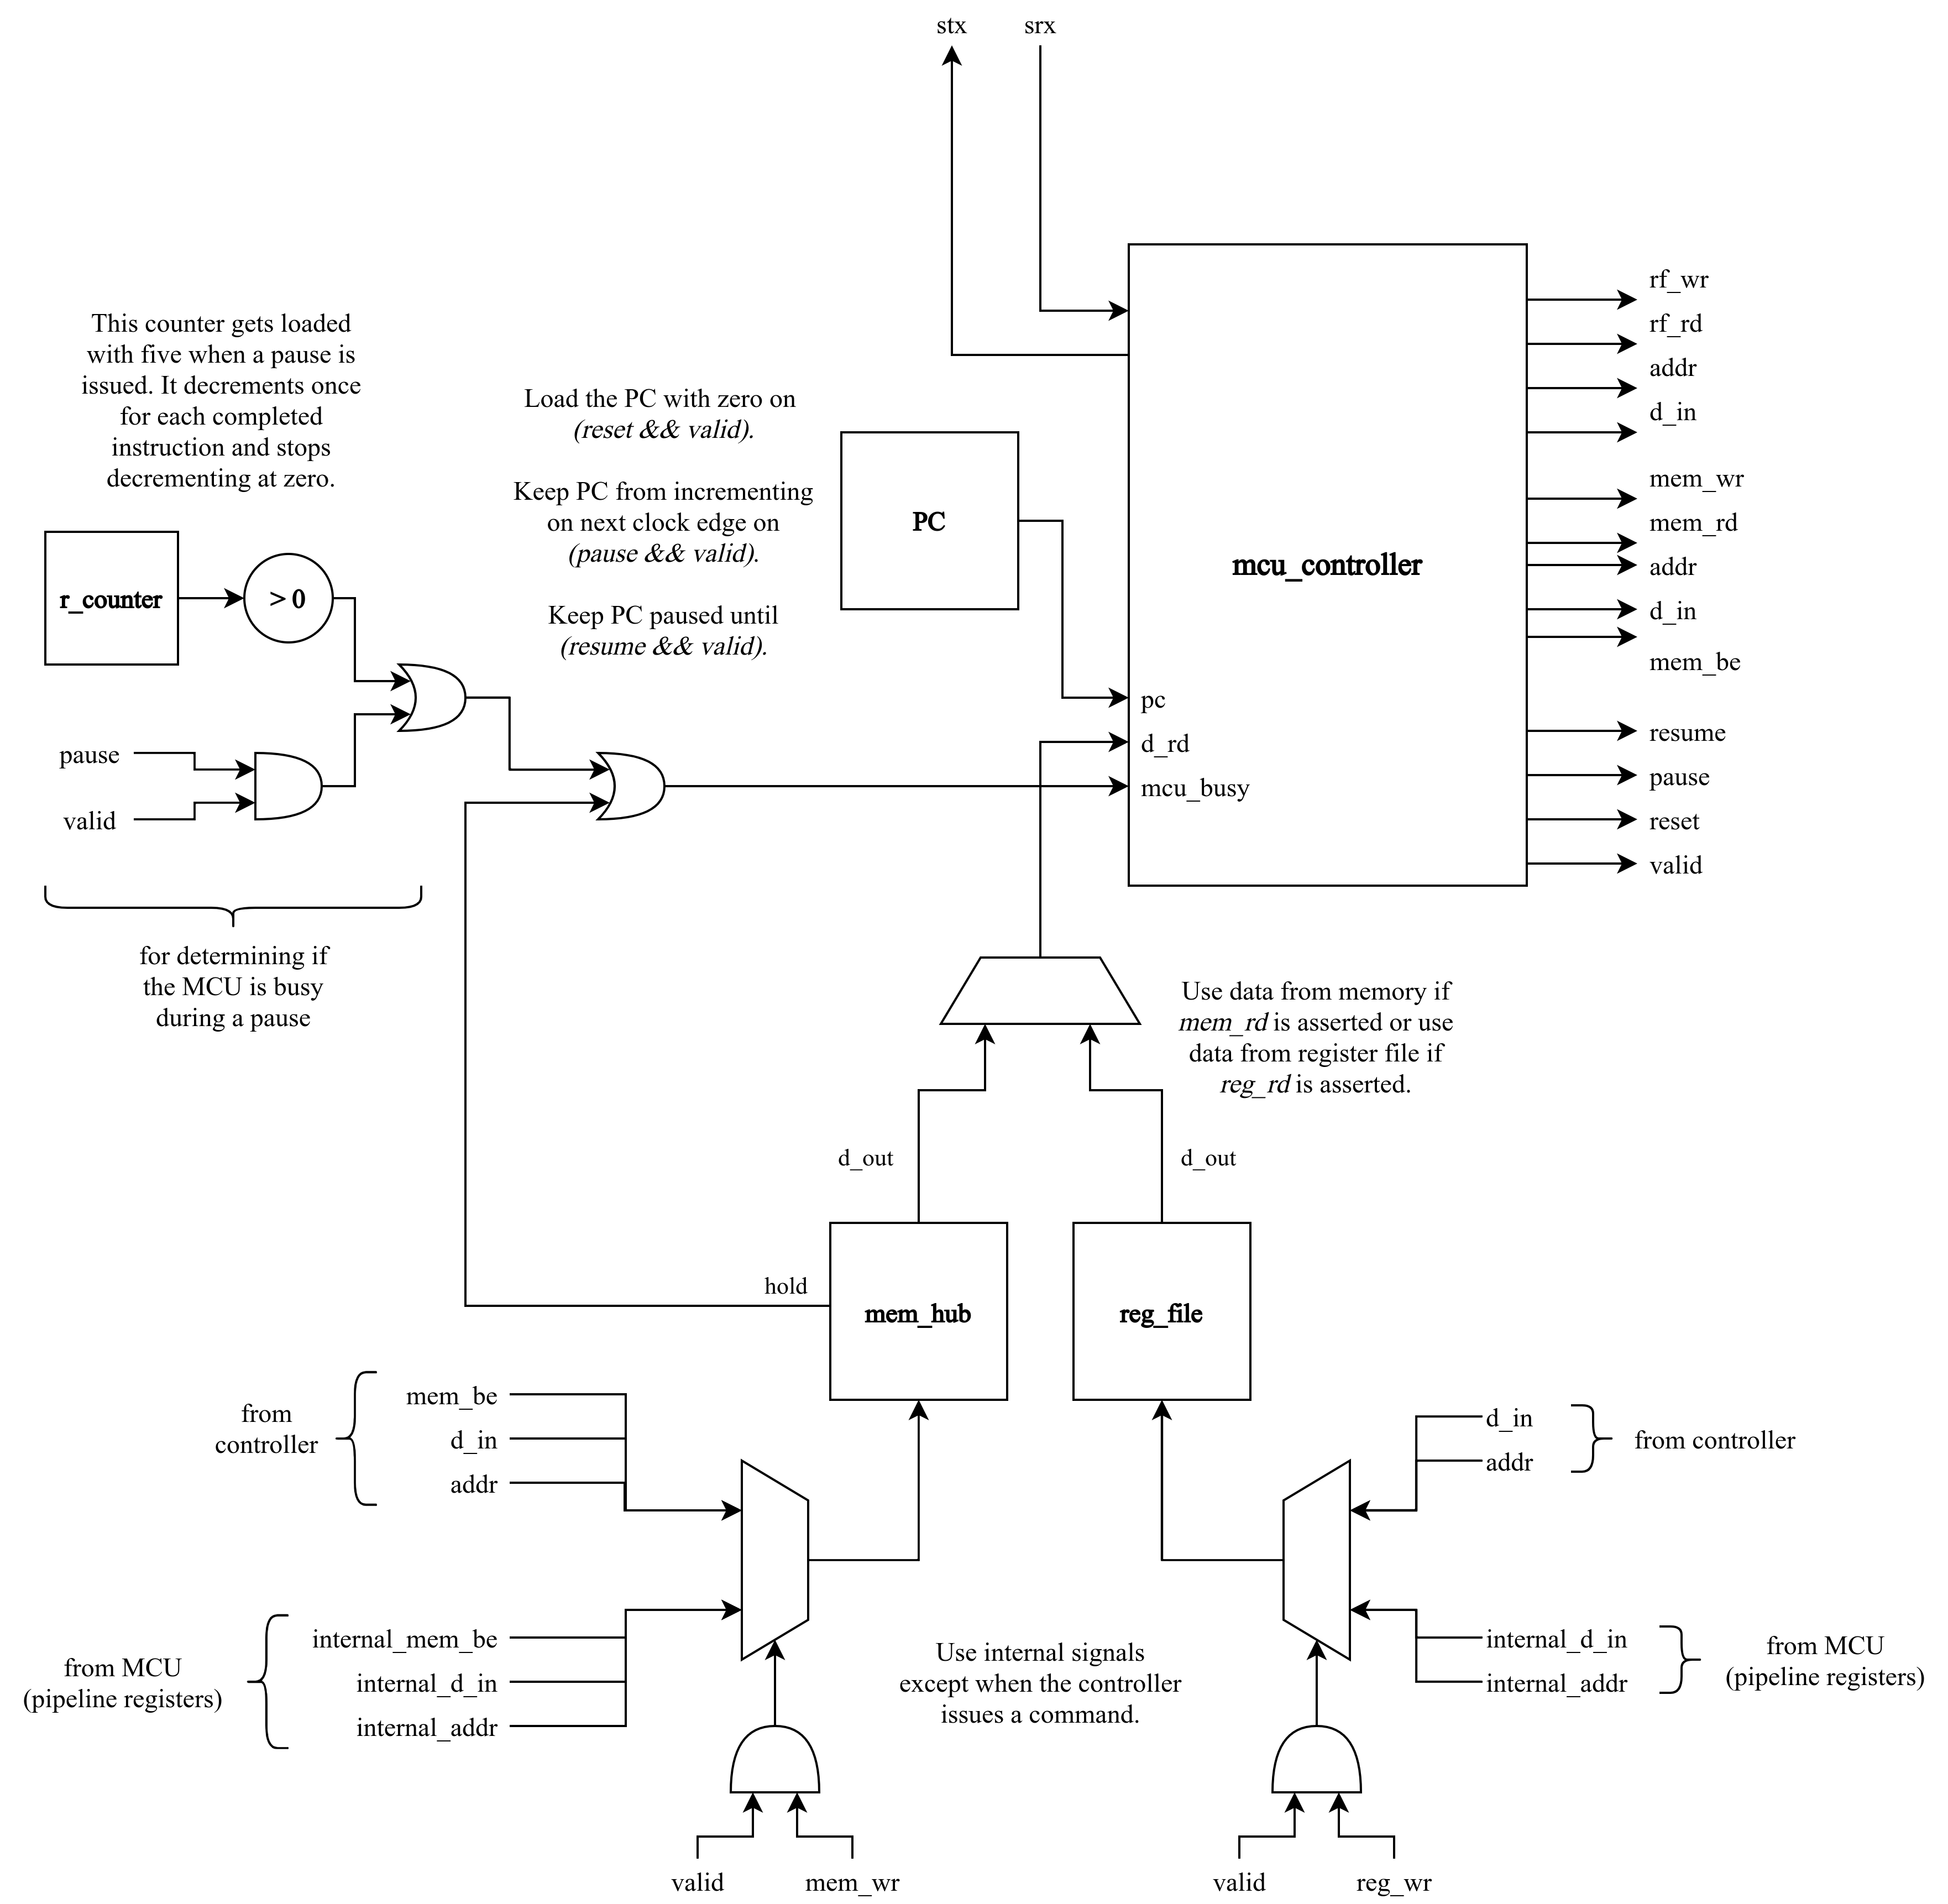
\includegraphics[width=\linewidth]{pipeline.png}
\end{figure}
\end{center}

\newpage
\section{Debug client}
The client is a GDB-inspired command line debugger. It supports many basic debugging functions and
programming the Otter without having to re-generate the bitstream.

\subsection{Installation}
Using and installing the debug client is very simple. To clone the source code, build, and install,
run the following command:

\begin{verbatim}
    git clone git@github.com:trmckay/riscv-uart-debugger.git
    cd riscv-uart-debugger
    ./install
\end{verbatim}

Follow the instructions in your terminal, and installation should be easy. Be sure to scan the
output of the installer for any warnings.

\subsection{Usage}
When installation is complete, launch the debugger with the command \emph{uart-db}. If you agree to
autodetect, it will automatically connect to the Otter. If you already know the location of your
serial port, you can launch the client with \emph{uart-db [device path]}. Once in the debugging shell,
enter \emph{h} or \emph{help} to output the help message.

\vspace*{\fill}
\begin{center}
    \noindent Contact Trevor McKay with questions.\\
    \href{mailto:trmckay@calpoly.edu}{trmckay@calpoly.edu}
\end{center}

\end{document}
